\documentclass[]{report}
\usepackage[]{fancyhdr}
\usepackage{listings}
\usepackage{multicol}
\usepackage{graphicx}
\usepackage[]{hyperref}
\usepackage{xcolor}
\usepackage[]{wrapfig}
\definecolor{codegreen}{rgb}{0,0.6,0}
\definecolor{codegray}{rgb}{0.5,0.5,0.5}
\definecolor{codepurple}{rgb}{0.58,0,0.82}


\lstdefinestyle{mystyle}{
	backgroundcolor=\color{white},   
	commentstyle=\color{codegreen},
	keywordstyle=\color{magenta},
	numberstyle=\tiny\color{codegray},
	stringstyle=\color{codepurple},
	basicstyle=\ttfamily\footnotesize,
	breakatwhitespace=false,         
	breaklines=true,                 
	captionpos=b,                    
	keepspaces=true,                 
	numbers=left,                    
	numbersep=5pt,                  
	showspaces=false,                
	showstringspaces=false,
	showtabs=false,                  
	tabsize=2
}

\lstset{style=mystyle}

\fancyhead{}
\fancyfoot{}



\lhead{\leftmark}
\rhead{
\includegraphics[height=30pt]{EHTP.jpg}}

\lfoot{Abdellah Radad}
\rfoot{\thepage}

\renewcommand{\footrulewidth}{0.4pt}
\pagestyle{fancy}

\fancypagestyle{titlepage}
{
	\fancyhf{}
	\setlength{\headheight}{50pt}
	\fancyhead[C]{
\includegraphics[height=50pt]{EHTP.jpg}}
	\renewcommand{\headrulewidth}{0pt}
	\renewcommand\footrulewidth{0pt}
}

\author{Abdellah Radad}
\title{Chaînes d'acquisition de données: Compte rendu 2}
\begin{document}
	\begin{titlepage}
		\thispagestyle{titlepage}
		\begin{center}
			\begin{LARGE}
				Shortest path algorithm applied to a Neo4j graph database
				using the JAVA programming language.
			\end{LARGE}
		\end{center}
		
		\vskip 300pt
		{\centering  \textbf{By} Abdellah Radad }\\
		{\centering  Electrical Engineering Department }	
	\end{titlepage}
	\newpage
	\tableofcontents
	\newpage
	\listoffigures
	
	\chapter{Introduction to Graph Databases}
	\newpage
	\section{Graph theory}
	In the mathematical sense, a graph is a set of nodes and vertices $G  =$\{$N,\epsilon$\} with N being a set of nodes and $\epsilon$ the set of edges.\\
	We generally distinguish between two types of graphs: directed graphs and undirected graphs
	

	\begin{figure}[!htb]
			\centering
			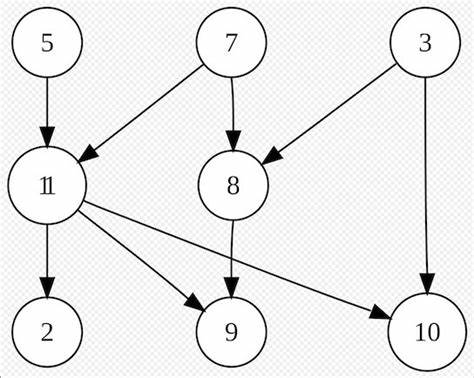
\includegraphics[width=0.5\textwidth]{directed_graph.jpg}
			\caption{Directed  graph}
	\end{figure}
	\begin{figure}[!htb]
			\centering
			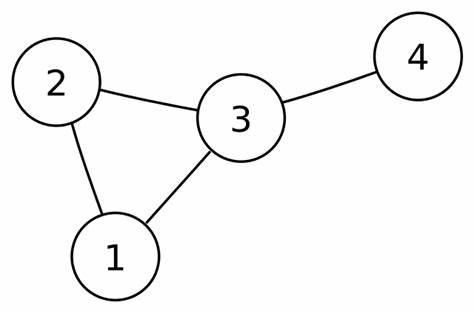
\includegraphics[width=0.5\textwidth]{undirected_graph.jpg}
			\caption{Undirected graph}
	\end{figure}
	
	Graph theory is a branch of mathematics that takes interest in the study of such mathematical structure, and during this project it will come in handy.
	\newpage
	\section{Graph Databases}
	\subsection{Introduction}
	Graph Databases are databases that make use of graphs to represent data points and the relations tying these data points together.
	
	Graph Databases are commonly used for highly connected data and are generally considered to emphasize less the contents of the data.
	
	Generally, data points are represented as nodes with the different relations between nodes being represented by edges.
	\begin{figure}[!htb]
		\centering
		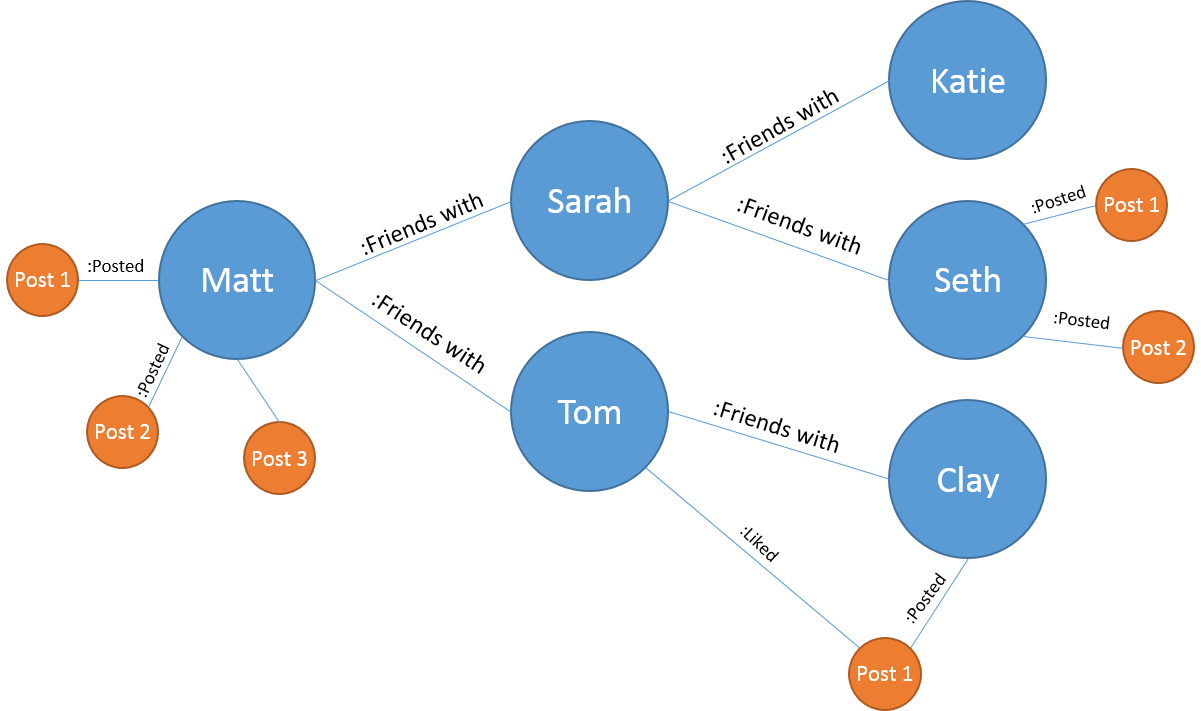
\includegraphics[width=1\textwidth]{graphDB.png}
		\caption{Example of a Graph Database}
	\end{figure}
	\subsection{Graph Databases vs. Relational Databases}
	While Relational Databases see more general use than Graph Databases, Graph Databases (or NoSQL Databases) present numerous advantages over the traditional Relational Databases, these advantages include but are not limited to:
	\begin{enumerate}
		\item A clearer representation of Relations and Many to Many relations.
		\item Low latency and better scaling.
		\item Faster response to complex queries and more performant insertions/deletions.
	\end{enumerate}
	These performance benefits are inherent to the graph structures, while we get all of those benefits we do suffer from a weaker data representation when compared with traditional SQL tables.
	\newpage
	\section{Neo4j}
	According to the Neo4j product brief, a Neo4j Graph Database is the market leading database that 
	empowers developers to create intelligent applications that 
	harness the rich relationships in your data and answer complex 
	questions with speed that no other database can match. 
	As the heart of the Neo4j Graph Data Platform, Neo4j Graph 
	Database helps enterprises across industries – life sciences, 
	utilities, financial services, cybersecurity, and many more – 
	uncover hidden insights in real time.\\
	Neo4j puts emphasis on the following points:
	\begin{itemize}
		\item  Fast Performance
		\item Unbounded Scale
		\item Developer Productivity
		\item Operational Trust
	\end{itemize} 
	That's why we're going to be using the Neo4j JAVA driver for our project.
	\newpage
	\chapter{Setting up the environment}
	\newpage
	\section{IDE and Build system}
	For this project we picked intelliJ IDEA as our IDE of choice. Running on fedora linux 37, with maven as our build system.
		\begin{figure}[!htb]
		\centering
		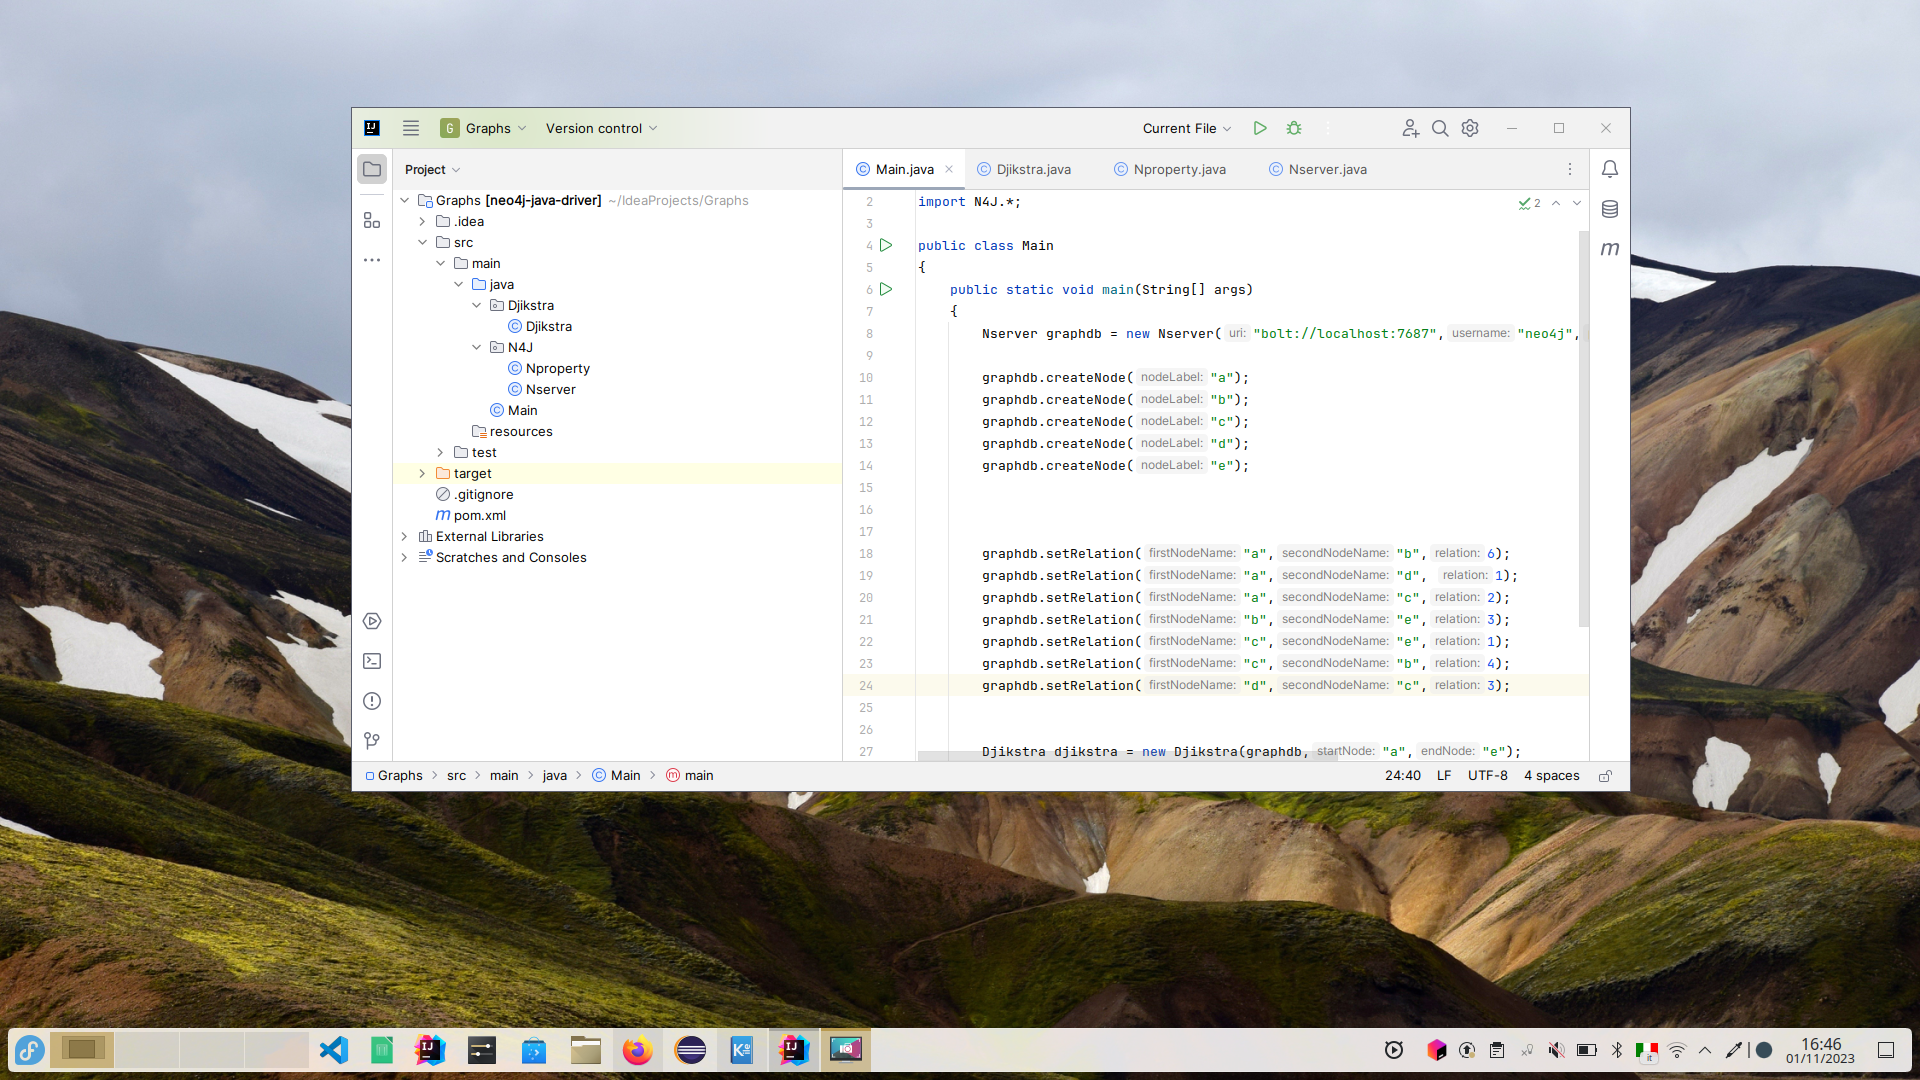
\includegraphics[width=1\textwidth]{intellij.png}
		\caption{Intellij IDEA}
	\end{figure}
	\newpage
	\subsection{Installing IntelliJ IDEA}
	To install IntelliJ IDEA, head over to the \href{https://www.jetbrains.com/toolbox-app/}{official JetBrains website} and install the intelliJ toolbox app or download it as an app image.\\
	\begin{figure}[!htb]
		\centering
		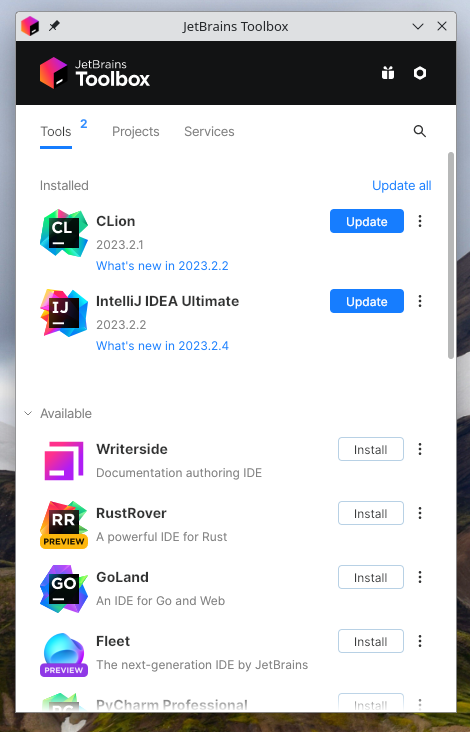
\includegraphics[width=0.5\textwidth]{intellij_toolbox.png}
		\caption{Intellij toolbox}
	\end{figure}

	If you dont have intelliJ IDEA Installed already it should show under the available section.\\
	Please note that JetBrains license all their products for free for students, so no software has been pirated in the making of this project.
	\newpage
	\section{Installing Neo4j}
	Similiarly to Intellij IDEA, the Neo4j desktop client is packaged as an appimage ready for use on linux.\\
	After creating an account on \href{https://neo4j.com/product/developer-tools/}{Neo4j's website} the package should be available to download with a limited license.\\
	\begin{figure}[!htb]
		\centering
		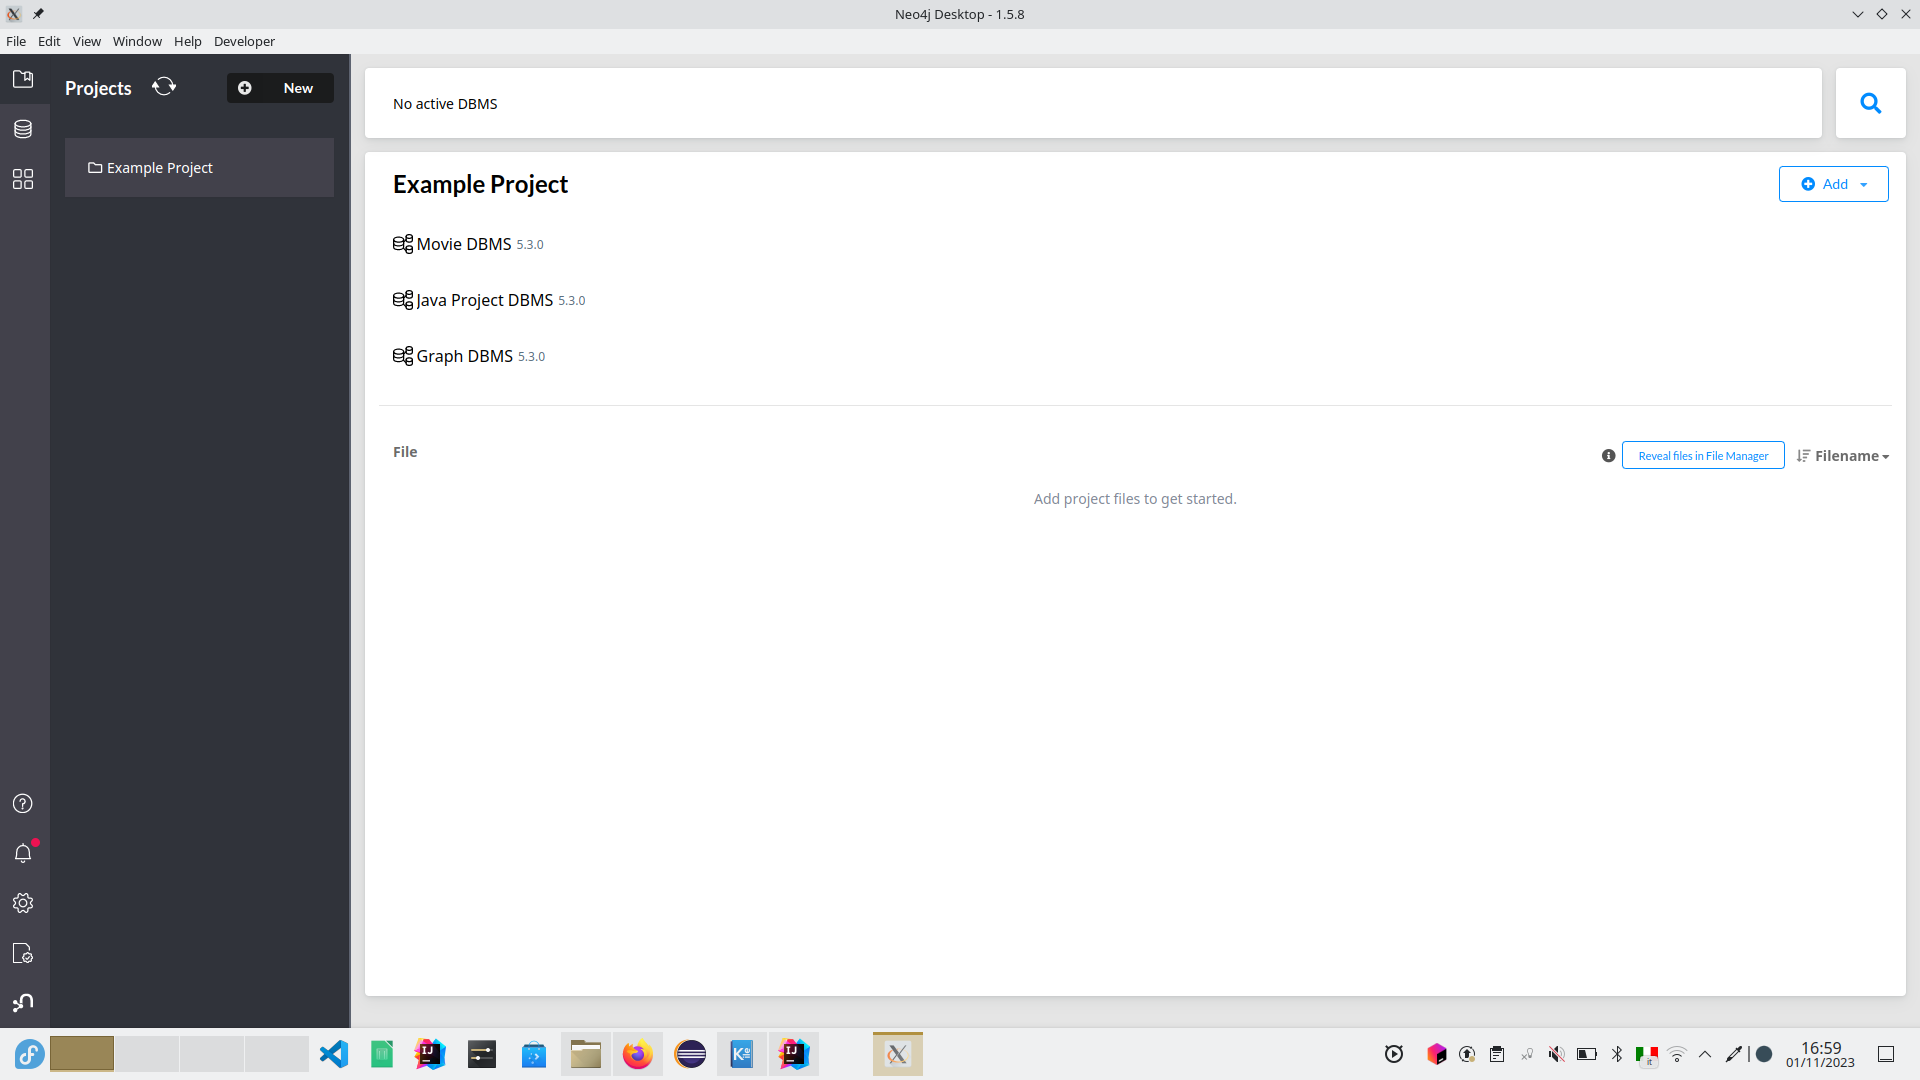
\includegraphics[width=1\textwidth]{neo4j_desktop.png}
		\caption{The Neo4j desktop client}
	\end{figure}
	\newpage
	\section{Installing Maven}
	Throughout this project, we will be using Maven as our build system, but before using it we need to first have a system wide install of the Maven build system.\\
	For Fedora linux 37, run the following command to install Maven:
	\begin{center}
	 \textbf{sudo dnf install maven}
	\end{center}
	for windows and other linux distributions, please consult \href{https://maven.apache.org/}{Apache Maven's official website} for platform specific install instructions.
	\newpage
	\section{Creating the project and installing the Neo4j Java Driver}
	When creating a new project under intelliJ IDEA, we must choose "Maven" as our build system.\\
	\begin{figure}[!htb]
		\centering
		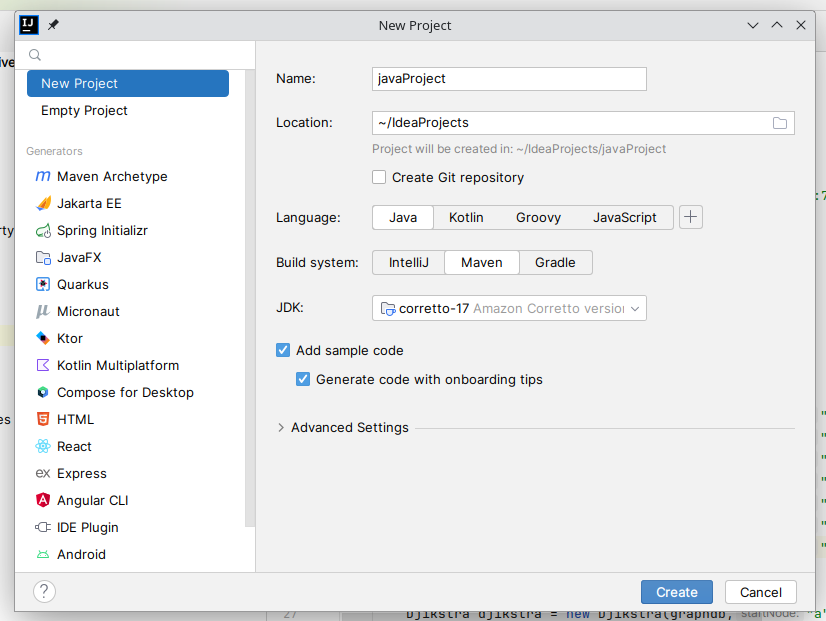
\includegraphics[width=1\textwidth]{new_project.png}
		\caption{Creating a new Maven project}
	\end{figure}

	With Maven selected we must add the following lines to the \textbf{pom.xml} file to include the Neo4j Java driver as a dependency in our project:\\
	\begin{lstlisting}[language=xml]
	<groupId>org.neo4j.driver</groupId>
    <artifactId>neo4j-java-driver</artifactId>
    <version>5.7.0</version>
    <dependencies>
        <dependency>
            <groupId>org.neo4j.driver</groupId>
            <artifactId>neo4j-java-driver</artifactId>
            <version>5.12.0</version>
        </dependency>
    </dependencies>
	\end{lstlisting}
\newpage
\chapter{Code and documentation}
On my \href{https://github.com/abdellah2288}{github} under the Graphs repository a fully functional version of the code alongside documentation generated using \textbf{Javadoc}
\end{document}
